\section{A Gaussian observation shared by the Riemann and Navier--Stokes settings}
\label{sec:gaussian-bridge}

The comparisons of the preceding sections are structural.  This section
and the next record a concrete construction instead: one family of
complex Gaussian observations is applied both to finite sets of zeros of
the completed zeta function and to the Fourier side of the
three-dimensional Navier--Stokes equations, and in
\Cref{sec:triad-bridge} also to the assignments of a CNF formula.  The
identities are elementary: they come from completing the square in a
Gaussian integral and from the linearity of the observation.  They are
proved without any of the conditional schemas of
\Cref{sec:foreclosure,sec:recognition}, and their formal proofs use
only the standard axioms (\Cref{app:formalization}).  What they show is
that a single observation family can be read on all three objects; they
do not show that the hypotheses of the three conditional closures
support one another.

\subsection{The observation}

Write \(\xi\in\mathbb R^{3}\) for the Fourier variable.  Following the
Navier--Stokes companion \cite{Tsiokos2026NavierStokes}, fix a Sobolev
index \(\gamma>5/2\) and represent a velocity field \(u\) by its
\emph{weighted Fourier state}
\(g(\xi)=(1+|\xi|^{2})^{\gamma/2}\hat u(\xi)\), an element of
\(L^{2}(\mathbb R^{3};\mathbb C^{3})\); the physical amplitude is
\(\hat u=(1+|\xi|^{2})^{-\gamma/2}g\).  The observations below are
applied to weighted states.  For a width
\(a>0\), a unit vector \(\theta\in\mathbb R^{3}\) and a complex centre
\(z\in\mathbb C\), put
\[
  w_{a,\theta,z}(\xi)
  =\exp\bigl(-a|\xi|^{2}+2az\langle\theta,\xi\rangle-az^{2}\bigr),
  \qquad
  \mathcal O_{a,\theta,z}(g)=\int_{\mathbb R^{3}}w_{a,\theta,z}(\xi)\,g(\xi)\,d\xi .
\]
For real \(z\) the window is the Gaussian
\(\exp(-a|\xi-z\theta|^{2})\) centred at \(z\theta\); complex \(z\) is
its analytic continuation in the centre.  We fix \(\theta=\theta_{\rm
axis}\), the first coordinate vector, whenever a single direction is
needed.

Let \(\nu>0\) be the viscosity and \(t>0\) a time, and put
\(b=4\pi^{2}\nu t\).  With the convention
\(\hat g(\xi)=\int g(x)e^{-2\pi i x\cdot\xi}\,dx\), the heat semigroup
\(e^{\nu t\Delta}\) acts on Fourier states, weighted or not, as
multiplication by \(e^{-b|\xi|^{2}}\).  Completing the square gives,
with \(\kappa=ab/(a+b)\),
\begin{equation}
\label{eq:joint-heat-kernel}
  N_{a,b}(z):=\int_{\mathbb R^{3}}w_{a,\theta,z}(\xi)\,e^{-b|\xi|^{2}}\,d\xi
  =\Bigl(\frac{\pi}{a+b}\Bigr)^{3/2}e^{-\kappa z^{2}},
\end{equation}
and, for every Fourier state \(g\),
\[
  \mathcal O_{a,\theta,z}\bigl(e^{\nu t\Delta}g\bigr)
  =e^{-\kappa z^{2}}\,
    \mathcal O_{a+b,\,\theta,\,az/(a+b)}(g).
\]

\subsection{The zero side}

Let \(\rho\) be a zero of the completed zeta function in the critical
strip \(0<\operatorname{Re}\rho<1\).  Its \emph{spectral coordinate} is
\[
  z_{\rho}=\operatorname{Im}\rho+i\bigl(\tfrac12-\operatorname{Re}\rho\bigr),
  \qquad\text{so that}\qquad
  \operatorname{Re}\bigl(z_{\rho}^{2}\bigr)
  =(\operatorname{Im}\rho)^{2}-\bigl(\operatorname{Re}\rho-\tfrac12\bigr)^{2}.
\]
By \eqref{eq:joint-heat-kernel}, the logarithmic excess
\[
  \ell_{a,b}(\rho)
  :=\log\frac{|N_{a,b}(z_{\rho})|}{(\pi/(a+b))^{3/2}}
        +\kappa\,(\operatorname{Im}\rho)^{2}
  =\kappa\,\bigl(\operatorname{Re}\rho-\tfrac12\bigr)^{2}
\]
is defined so as to isolate the horizontal distance of \(\rho\) from
the critical line.

The map \(J(\rho)=1-\bar\rho\) is the reflection in the critical line;
it sends zeros to zeros by the functional equation and the reality of
the completed zeta function on the real axis.  A \emph{reflected
window} is a finite set \(W\) of distinct zeros in the strip with
\(J(W)=W\); multiplicities enter only through the weights.
Let \(m:W\to\mathbb N\) be weights with \(m\circ J=m\), and put
\[
  E^{\mathrm{heat}}_{a,\nu,t}(W)=\sum_{\rho\in W}m(\rho)\,\ell_{a,b}(\rho),
  \qquad
  v_{W}(\rho)=\sqrt{m(\rho)}\,\bigl(\operatorname{Re}\rho-\tfrac12\bigr),
  \qquad
  L_{W}x=\sum_{\rho\in W}x_{\rho}
\]
for \(x\in\mathbb R^{W}\).  In the language of the adequacy-residual
companion \cite{Tsiokos2026XiCompanion}, the residual of the identity
target against the probe \(L_{W}\), at identity audit energy, is the
orthogonal projection \(\Xi(L_{W})\) of \(\mathbb R^{W}\) onto
\(\ker L_{W}\).  The reflection reverses the sign of each displacement
and preserves the weights, so \(L_{W}v_{W}=0\) and
\(\Xi(L_{W})v_{W}=v_{W}\).  Hence
\begin{equation}
\label{eq:joint-heat-xi}
  E^{\mathrm{heat}}_{a,\nu,t}(W)
    =\kappa\sum_{\rho\in W}m(\rho)\bigl(\operatorname{Re}\rho-\tfrac12\bigr)^{2}
  =\frac{ab}{a+b}\,\bigl\|\Xi(L_{W})v_{W}\bigr\|^{2}.
\end{equation}
We call \(\|\Xi(L_{W})v_{W}\|^{2}\) the \emph{residual charge} of the
window; it vanishes exactly when every zero of positive weight in \(W\)
lies on the critical line.  The first equality holds for any finite set
of points of the strip with any nonnegative weights.  On the zero side
the residual projection does no work: the reflection hypotheses place
\(v_{W}\) in \(\ker L_{W}\), so the residual charge is just
\(\|v_{W}\|^{2}\).  The projection matters on the SAT side of
\Cref{sec:triad-bridge}, where native and residual channels differ.

\subsection{The fluid side}

Let \(g_{0}\) be a weighted Fourier state.  A time
\(t\ge0\) is \emph{admissible} for \(g_{0}\) if the mild formulation of
the Navier--Stokes equations with data \(g_{0}\) has a solution on
\([0,t]\) in the class of weighted states of index \(\gamma\) used in
\cite{Tsiokos2026NavierStokes}; when the physical amplitude of \(g_{0}\)
is that of a real, divergence-free field, positive admissible times
exist by local existence.  On admissible times the maximal mild solution
satisfies, in weighted coordinates,
\[
  g(t)=e^{\nu t\Delta}g_{0}-\mathcal D[g](t),
\]
where \(\mathcal D[g](t)\) is the nonlinear heat--Duhamel term: the
integral over \([0,t]\) of the heat semigroup applied to the
Leray-projected convection term \(P(u\cdot\nabla)u\), written in the
weighted coordinates and with the normalization of the Navier--Stokes
companion \cite{Tsiokos2026NavierStokes}, where the convection term is
carried at Sobolev weight \(\gamma-1\) and the heat semigroup supplies
the missing derivative.  Applying the linear observation to this equation
gives
\begin{equation}
\label{eq:joint-navier-return}
  \mathcal O_{a,\theta,z}(g(t))
  +\mathcal O_{a,\theta,z}(\mathcal D[g](t))
  =\mathcal O_{a,\theta,z}(e^{\nu t\Delta}g_{0}).
\end{equation}
This is the mild equation, observed: it keeps the nonlinear term and
says nothing about its size.

\begin{theorem}[Joint Gaussian observation and source return]
\label{thm:joint-gaussian-return}
Let \(a>0\), \(\nu>0\), \(\gamma>5/2\), let \(g_{0}\) be a weighted
Fourier state, and let \(t>0\) be admissible for \(g_{0}\); put
\(b=4\pi^{2}\nu t\) and \(\kappa=ab/(a+b)\).  Let \(W\) be a reflected
window with weights \(m:W\to\mathbb N\) satisfying \(m\circ J=m\), and
let \(\rho\in W\).  Then:
\begin{enumerate}
\item the heat excess of the window is the residual charge times
  \(\kappa\), as in \eqref{eq:joint-heat-xi};
\item the heat observation at the zero has the value
  \(N_{a,b}(z_{\rho})=(\pi/(a+b))^{3/2}e^{-\kappa z_{\rho}^{2}}\);
\item the maximal mild solution satisfies \eqref{eq:joint-navier-return}
  with \(\theta=\theta_{\rm axis}\) and \(z=z_{\rho}\);
\item \(m(\rho)(\operatorname{Re}\rho-\frac12)^{2}\le
  \|\Xi(L_{W})v_{W}\|^{2}\).
\end{enumerate}
\end{theorem}

\begin{proof}
Parts (1) and (2) are \eqref{eq:joint-heat-kernel} and the computation
leading to \eqref{eq:joint-heat-xi}.  Part (3) is the observation of the
mild equation.  Part (4) holds because the charge is a sum of
nonnegative terms, one of which is \(m(\rho)(\operatorname{Re}\rho-\frac12)^{2}\).
\end{proof}

Only part (3) involves \(\gamma\), \(g_{0}\) and the admissibility of
\(t\); parts (1), (2) and (4) concern the scalar kernel and hold for
all \(a,\nu,t>0\).  The theorem collects four elementary facts; its
point is that one observation family is read on both objects.

\begin{figure}[tbp]
\centering
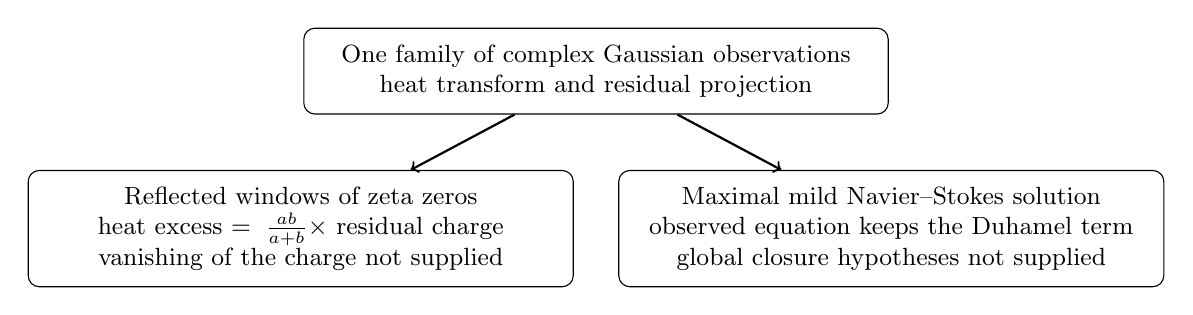
\begin{tikzpicture}[every node/.style={draw,rounded corners,
  align=center,inner sep=6pt,font=\small}]
\node[text width=7.0cm] (obs) at (0,2.0)
  {One family of complex Gaussian observations\\
   heat transform and residual projection};
\node[text width=6.5cm] (rh) at (-3.75,0)
  {Reflected windows of zeta zeros\\
   heat excess $=\frac{ab}{a+b}\times$ residual charge\\
   vanishing of the charge not supplied};
\node[text width=6.5cm] (ns) at (3.75,0)
  {Maximal mild Navier--Stokes solution\\
   observed equation keeps the Duhamel term\\
   global closure hypotheses not supplied};
\draw[->,thick] (obs) -- (rh);
\draw[->,thick] (obs) -- (ns);
\end{tikzpicture}
\caption{One observation construction read on two objects.  The lower
line of each box names what the identities do not provide.}
\label{fig:joint-observation-branches}
\end{figure}

The same observation can be applied after the high-frequency residual
projection of the Navier--Stokes companion, which gives a projected
form of \eqref{eq:joint-navier-return} with the projected Duhamel term
still present.  It can also be applied to three mild solutions at once,
one for each coordinate direction; this three-solution \emph{frame} is
the version used in \Cref{sec:triad-bridge}.

\subsection{What each conditional closure still needs}

For fixed \(a,\nu,t>0\), let \(\mathcal A_{a,\nu,t}\) be the statement
that the heat excess vanishes, with unit weights, on every canonical
window, the set of zeros in the strip at distance at most \(n\) from
\(\frac12\) (\(n\in\mathbb N\)).  These windows are reflected and
exhaust the zeros in the strip, so by \eqref{eq:joint-heat-xi}
\[
  \mathcal A_{a,\nu,t}
  \quad\Longleftrightarrow\quad
  \text{the Riemann hypothesis}.
\]
The equivalence is a reformulation, and it measures the strength of the
premise \(\mathcal A_{a,\nu,t}\): the premise is the Riemann hypothesis.
The Gaussian identities supply no prime-side or trace-formula argument
for it.  The Riemann-hypothesis companion \cite{Tsiokos2026RH} follows a
different conditional route, in which a supplied Selberg recognition
source together with an identification with the classical zeros implies
the Riemann hypothesis.

On the fluid side, the Navier--Stokes companion
\cite{Tsiokos2026NavierStokes} proves two conditional returns, for
positive viscosity and real divergence-free initial data in
\(H^\gamma(\mathbb R^3)\), \(\gamma>5/2\).  A spectral closure hypothesis
on the maximal mild solution gives a global lifespan and a classical
solution.  A physical-window closure, for some \(0<\varepsilon<1\), asks for
finite Fourier shell witnesses whose amplitude and reconstruction
bounds satisfy \(2^{-\varepsilon j}(R_{t,j}+e_{t,j})\le b_T(t)\) on the
shells of the Bradshaw--Grujić window, with a majorant
\(b_T\in L^{2/(1-\varepsilon)}(0,T)\) for every possible preterminal
horizon \(T\); it gives a global strong mild solution only
together with a terminal-divergence input of Bradshaw--Grujić type for
the same maximal path and windows; that input is assumed there, not
derived.  These hypotheses concern
high frequencies, reconstruction and long times; the zero-side premise
concerns horizontal displacement of zeros.  Neither is derived from the
other through the shared observation.  A common source theorem would
have to supply both, and none is proved here.
